\documentclass[11pt]{article}
\usepackage{amsmath}
\usepackage{amssymb}
\usepackage{graphicx}
\usepackage{enumerate}
\usepackage{hyperref}
\usepackage{tikz}

\pagestyle{plain}
\title{CSCI 4302/5302 Advanced Robotics\\
Assignment 5.1: Discrete Bayes Filter}
\author{Due: April 4th 2025}
\date{}

\begin{document}
\maketitle

\section{Introduction}
In this assignment, you will implement a discrete Bayes filter for robot localization in a grid world environment. The Bayes filter is a fundamental algorithm in probabilistic robotics that maintains a belief state over possible robot locations and updates this belief based on actions and measurements.

\section{Environment Description}
The robot operates in a discrete grid world environment with the following properties:

\subsection{Grid World}
\begin{itemize}
    \item The environment is represented as a 2D grid of cells
    \item Each cell is either free (0) or occupied by an obstacle (1)
    \item The robot's state consists of its position (i,j) in the grid
    \item The robot's heading is discretized into four directions:
        \begin{itemize}
            \item 0: facing right (positive x)
            \item 1: facing up (positive y)
            \item 2: facing left (negative x)
            \item 3: facing down (negative y)
        \end{itemize}
\end{itemize}

\section{Motion Model}
The robot can execute three types of actions:

\subsection{Action Space}
\begin{itemize}
    \item Forward (action = 0): Move one cell in the current heading direction
    \item Turn Right (action = 1): Rotate 90 degrees clockwise
    \item Turn Left (action = 2): Rotate 90 degrees counterclockwise
\end{itemize}

\subsection{Motion Uncertainty}
The motion model includes uncertainty in the following ways:
\begin{itemize}
    \item Motion noise: There is a probability \texttt{motion\_noise} (default: 0.2) that an action fails:
        \begin{itemize}
            \item For forward motion: The robot stays in place
            \item For turns: The robot still changes heading
        \end{itemize}
    \item Heading uncertainty: The robot's true heading is unknown, modeled as a uniform distribution over all four directions
    \item Collision handling: If a forward action would result in collision with an obstacle or wall, the robot stays in place
\end{itemize}

\subsection{Motion Model Equations}
For a forward action, the transition probability is:
\[
p(x_t|x_{t-1}, u_t=\text{forward}) = \begin{cases}
1-p_{\text{noise}} & \text{if } x_t \text{ is valid forward cell} \\
p_{\text{noise}} & \text{if } x_t = x_{t-1} \\
0 & \text{otherwise}
\end{cases}
\]

For turn actions, the transition probability is:
\[
p(x_t|x_{t-1}, u_t=\text{turn}) = \begin{cases}
1 & \text{if } x_t = x_{t-1} \\
0 & \text{otherwise}
\end{cases}
\]

\section{Measurement Model}
The robot is equipped with a simple beam-based sensor system:

\subsection{Sensor Configuration}
\begin{itemize}
    \item Four beam sensors, one in each cardinal direction relative to the robot's heading
    \item Each beam measures the distance to the nearest obstacle or wall
    \item Measurements are corrupted by Gaussian noise with standard deviation \texttt{sensor\_noise\_std}
\end{itemize}

\subsection{Measurement Process}
For each beam:
\begin{itemize}
    \item Cast a ray from the robot's position in the beam's direction
    \item Count cells until hitting an obstacle or wall
    \item Add Gaussian noise to the count
    \item Return the noisy distance measurement
\end{itemize}

\subsection{Measurement Model Equations}
The measurement likelihood for a single beam is:
\[
p(z_i|x) = \begin{cases}
1-p_{\text{noise}} & \text{if } |z_i - \hat{z}_i(x)| < \text{tolerance} \\
p_{\text{noise}} \cdot \frac{1}{1 + |z_i - \hat{z}_i(x)|} & \text{otherwise}
\end{cases}
\]
where:
\begin{itemize}
    \item $z_i$ is the actual measurement for beam $i$
    \item $\hat{z}_i(x)$ is the expected measurement from state $x$
    \item $p_{\text{noise}}$ is the measurement noise parameter
    \item tolerance is the acceptable difference threshold
\end{itemize}

The total measurement likelihood is:
\[
p(z|x) = \prod_{i=1}^4 p(z_i|x)
\]

\section{Implementation Tasks}

\subsection{Prediction Step}
Implement the \texttt{predict(action)} method in \texttt{bayes\_filter.py}:
\begin{itemize}
    \item Apply motion model to current belief state
    \item Handle uncertainty in robot motion
    \item Account for different action types
    \item Ensure proper probability normalization
\end{itemize}

\subsection{Update Step }
Implement the \texttt{update(readings)} method in \texttt{bayes\_filter.py}:
\begin{itemize}
    \item Incorporate sensor measurements into belief state
    \item Handle measurement noise
    \item Process beam readings correctly
    \item Normalize posterior distribution
\end{itemize}

\subsection{Analysis and Visualization }
\begin{itemize}
    \item Use the scripts in the test directory to evaluate if your filter is working
    \item You can visualize using the visualizer

\end{itemize}

\section{Getting Started}

\subsection{Installation}
Install the package with student dependencies:
\begin{verbatim}
pip install -e ".[assignment1]"
\end{verbatim}

\subsection{Code Structure}
The template file \texttt{bayes\_filter.py} contains:
\begin{itemize}
    \item Class definition with required methods
    \item Docstrings explaining expected behavior
    \item TODO comments marking implementation points
    \item Helper functions for common operations
    \item \emph{Only} change code in the functions with TODO docstrings in the Bayes Filter class.
\end{itemize}



\subsection{Testing}
Run the provided test suite:
\begin{verbatim}
pytest tests/test_bayes_filter.py -v
\end{verbatim}

\section{Submission Instructions}
Create a branch on github with the codebase and your implementations. Provide a link to the branch.
https://github.com/gyanigk/Advanced-Robotics.git

\begin{figure}[H]
    \centering
    \begin{minipage}[t]{1.0\textwidth}
        \centering
        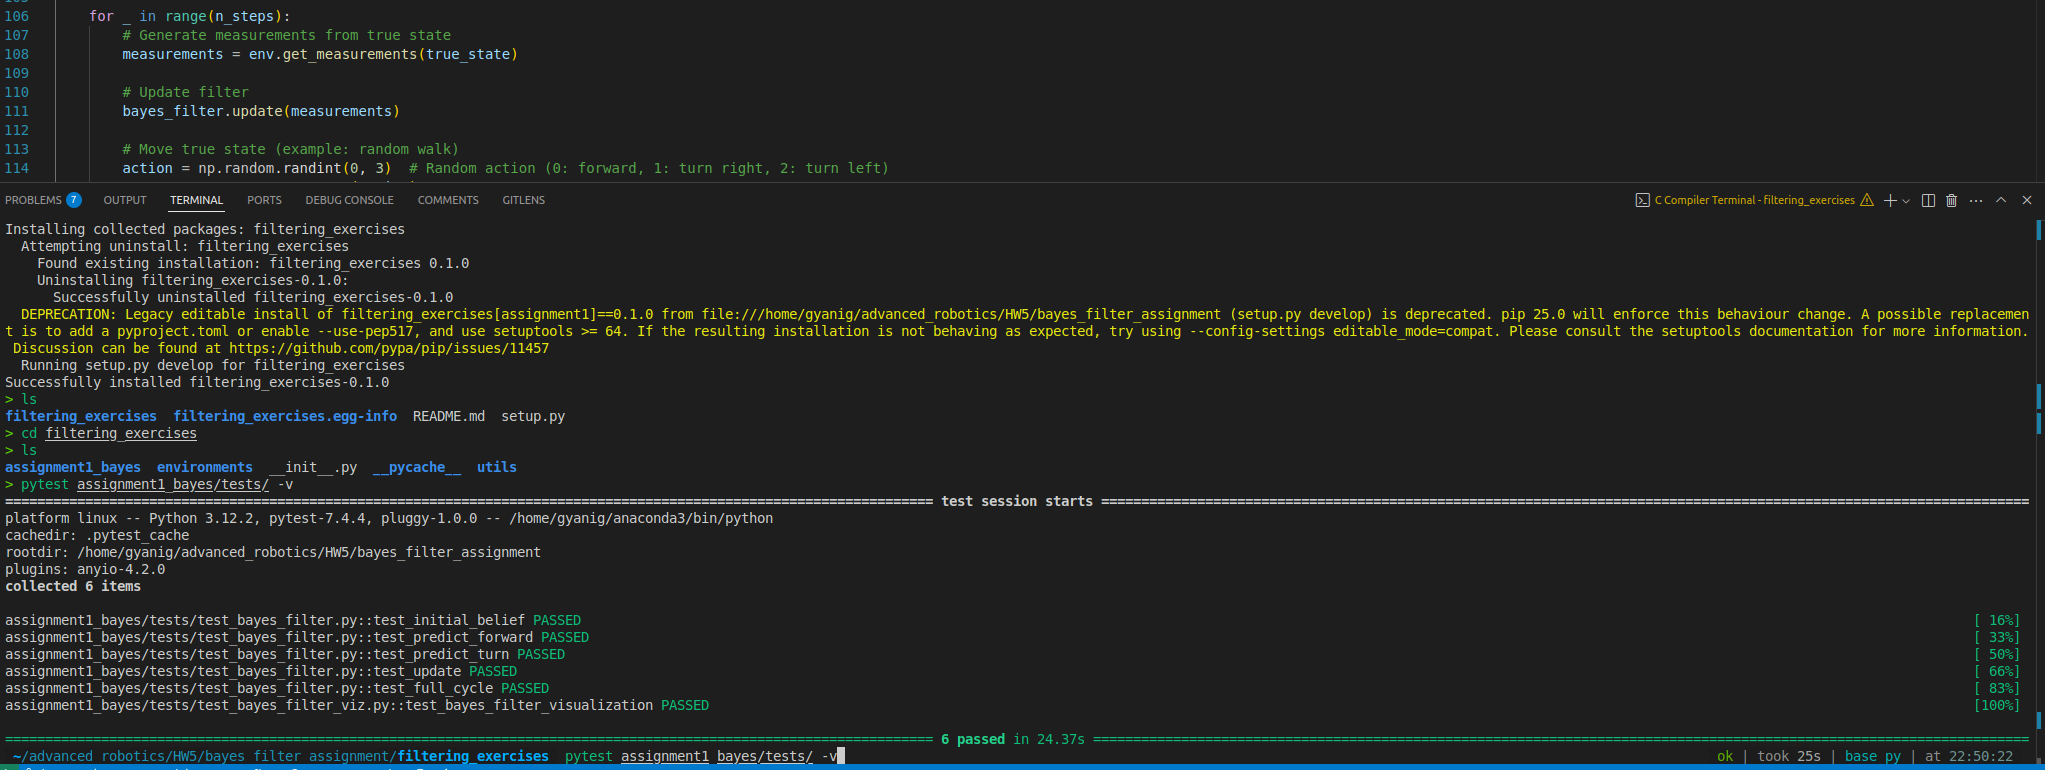
\includegraphics[width=\textwidth]{/home/gyanig/advanced_robotics/HW5/bayes_filter_assignment/filtering_exercises/assignment1_bayes/writeup/All_test_pass.png}
        \caption{All tests passed}
        \label{fig:gridworld_v0_det_vi}
    \end{minipage}
\end{figure}



\end{document} 